\chapter{Classification of ILP systems}\label{chap:classification_of_ilp_systems}

In the chapter \nameref{chap:issues_in_ilp} we analysed the central issues in ILP by providing a brief explanation of an importance of an issue and a list of the properties defining an issue. In this chapter we classify ILP systems and theoretical frameworks based on the use of the defining properties to approach solving a particar issue.

We will define an ILP task $I \mapsto O$ by its space of possible inputs $I$ and the decription of the desired output $O$. Thus an ILP task is a \emph{function problem} as opposed to a decision problem. We think of an ILP system solving such an ILP task as an \emph{algorithm} computing the function $I \mapsto O$.

\section{ILP task definition}
In \nameref{sec:ilp_task_definition} of the chapter \nameref{chap:issues_in_inductive_logic_programming} we presented machine learning problems: generalization and explanatory induction; together with the properties expressivity, positive examples, negative examples, semantics.

Although on the surface there may seem to be a standard definition of an ILP task, in this section we demonstrate that when specifying an ILP task completely, each ILP system classified solves a different learning problem. This mutual incompatibility has a major impact how we can assess, compare and classify ILP systems.

We explain the importance of defining an ILP task completely, present building blocks for a definition of an ILP task, construct an ILP definition for each ILP system, classify the ILP systems based on an ILP task they solve and lastly provide a generalized unifying definition of an ILP task for all assessed ILP systems to lay the ground for their comparisons and classification in the subsequent chapters.

\subsection{Importance of complete definitions}
Since an ILP task is a function problem $f:I \mapsto O$ for a specified input $I$ and a corresponding output $O$, its incomplete definition may not specify a \emph{unique deterministic function} $f$. An example of an incomplete definition is explanatory induction: given $I=\langle B, E \rangle$ find a correct $O=H$, i.e. satisfying
$E \in Cn(B \cup H)$ and $false \not\in Cn(B \cup H)$.
\begin{exmp}\label{explanatory_induction_definition_incompleteness}
Let $E=\{mortal(aristotle)\}$, $B=\{man(aristotle)\}$,
$H_1=E$, $H_2=\{mortal(aristotle) \leftObjectImplies man(aristotle)\}$.
Then both $H_1$, $H_2$ are correct hypotheses explaining $E$ from $B$. Therefore there are at least 2 different functions $\langle B, E \rangle \mapsto H_1$ and
$\langle B, E \rangle \mapsto H_2$ specifying the output $O=H$.
\end{exmp}

The importance of an issue of an incomplete definition becomes apparent when defining a non-ILP function problem as our mind is not biased towards the acceptance of the incompleteness of a definition encountered in the ILP literature.

\begin{exmp}
Define a function problem $f:I \mapsto O$ by given an odd number, find an even number. Then constant functions $f_2:I \mapsto 2$, $f_4:I \mapsto 4$, ..., functons $g_1:I \mapsto I+1$, $g_3:I \mapsto I+3$ and many others are compatible with an incomplete definition of a function $f$. However, when the definition of a function problem is completed to given an odd number $I$ to find smallest even number greater than $I$, then unambiguously $f=g_1$.
\end{exmp}

Not specifying an ILP task completely may result in designing an ILP system solving a different function problem than the one intended.

\subsection{Buildings blocks of ILP task definition}\label{subsec:building_blocks_of_ilp_task_definition}
In this subsection we define an ILP task definition, instantiate the definition with an ILP task of generalization, extend the definition of generalization by the notions encountered in ILP tasks of ILP systems we classify. The objective of this subsection is to enumerate the building blocks of an ILP task definition and the rules that make the definition more complete from which we can construct definitions of ILP tasks and classify their respective ILP systems later.

\begin{defn}\label{ilp_task_definition}
An \emph{ILP task definition} is a tuple $D=\langle f, dom(f), cod(f), R \rangle$ where a (possibly non-deterministic) function $f$ is called an \emph{ILP task}, $dom(f)$ is a set of \emph{inputs} vectors
$I=\langle \overrightarrow{i} \rangle$, $cod(f)$ is a set of \emph{output} vectors $O=\langle \overrightarrow{o} \rangle$ and $R$ is a set of rules (logical sentences) defining $f$,
i.e. $O \in f(I) \iff R \cup \{O \in f(I)\} \not\models false$ for a classical consequence operator $\models$. A vector component of an input(output) vector $\overrightarrow{i}$($\overrightarrow{o}$) is called an \emph{input component}(\emph{output component}) of an ILP task $f$. A \emph{structure component} of an ILP task is its input or output component. A \emph{rule} of an ILP task is a formula $\phi \in R$.
\end{defn}

\begin{remark}
We will often specify $R$ only by its subset of sentences and the rest will be specified informally or expected from the reader to be deduced from the context in order to avoid unnecessarily long specifications of $R$ and the lost of the focus. We may specify directly a possible input vector $I$ without specifying $dom(f)$ explicitly, it is be understood that $dom(f)$ is a set of all such input vectors $I$. Similarly, $cod(f)$ is a set of all possible output vectors $O$. The notation is abused for vectors with one element, e.g. $H=\langle H \rangle$.
\end{remark}

\begin{exmp}
The definition of explanatory induction is $D=\langle f, dom(f), cod(f), R \rangle$ where $I=\langle B, E \rangle$, $O=H$, $R=\{E \subseteq Cn(B \cup H), false \not\in Cn(B \cup H)\}$ for some consequence operator $Cn$. Input components of explanatory inductions are $B, E$. A hypothesis $H$ is an output component of explanatory induction.
\end{exmp}

\subsubsection{Completeness of definitions of ILP task}
By the example \fullref{explanatory_induction_definition_incompleteness} the definition of explanatory induction does not specify a unique deterministic ILP task, we say such a definition is incomplete.

\begin{defn}
A definition $D=\langle f, dom(f), cod(f), R \rangle$ is a \emph{complete ILP task definition} iff $f:I \mapsto O$ is deterministic. $D$ is \emph{incomplete} iff $D$ is not complete.
\end{defn}

Since an incomplete definition results in an ambiguous ILP task definition it will be in our interest to make the definitions more complete by introducing additional rules defining an ILP task.

\begin{defn}
Let $f:X \mapsto Y$ be a (possibly non-deterministic) function, we say that a (possibly non-deterministic) function $g:X \mapsto Y$ is a \emph{possible function} of $f$ iff
$\forall x \in X. g(x) \subseteq f(x)$. We denote the set of all possible functions of $f$ by $\Box f$.
\end{defn}

\begin{remark}
The only possible function of a deterministic function is the function itself, i.e. $\Box f = \{f\}$.
\end{remark}

\begin{defn}
A definition $D_1=\langle f_1, dom(f_2), cod(f_2), R \rangle$ is \emph{more complete} than the definition $D_2=\langle f_1, dom(f_2), cod(f_2), R \rangle$ iff
$f_2$ is a possible function of $f_1$.
\end{defn}

\begin{corollary}\label{corollary_more_complete_1}
Let $D_1=\langle f_1, \mathcal{I}, \mathcal{O}, R_1 \rangle$, $D_2=\langle f_2, \mathcal{I}, \mathcal{O}, R_2 \rangle$ be definitions of an ILP task.
If $R_2 \models R_1$, then $D_2$ is more complete than $D_1$.
\end{corollary}

\begin{proof}
Follows directly from the definitions.
\end{proof}

\subsubsection{Extension of ILP task definition}
To provide a more accurate and complete specification of an ILP task, its definition can be extended.

\begin{defn}\label{definition_ilp_task_definition_extension}
Let $D_1=\langle f_1, \mathcal{I}_1, \mathcal{O}_1, R_1 \rangle$ be a definition of an ILP task. A definition $D_2=\langle \mathcal{I}_2, \mathcal{O}_2, R_2 \rangle$ is an \emph{input component extension}(\emph{output component extension}) of a definition $D_1$ iff $\langle \overrightarrow{i_1} \rangle \subset \langle \overrightarrow{i_2} \rangle$. $D_2$ is a \emph{component extension} of $D_1$ iff $D_2$ is an input or output component extension of $D_1$. $D_2$ is a \emph{rule extension} $D_1$ iff $R_1 \subset D_2$. $D_2$ is an \emph{extension}(or an \emph{extended definition}) of $D_1$ iff $D_2$ is a component or rule extension of $D_1$.
A component $i \in \langle \overrightarrow{i_2} \rangle \setminus \langle \overrightarrow{i_1}$ with its set is an \emph{extending input component} of $D_2$ for $D_1$.
A component $o \in \langle \overrightarrow{o_2} \rangle \setminus \langle \overrightarrow{o_1}$ is an \emph{extending output component} of $D_2$ for $D_1$.
A component is an \emph{extending component} iff it is an extending input component or an extending output component.
A rule $r \in R_2 \setminus R_1$ is an \emph{extending rule} of $D_2$ for $D_1$.
\end{defn}

\begin{remark}
An extension of an ILP task definition defines a different ILP task.
\end{remark}

\begin{remark}
\emph{Extending rules of a component} are the rules which define the component (i.e. rules containing the symbols present in the denotation of the of the component). When a definition is extended by an extending component, the corresponding extending rules of an extending component need to be added as extending rules to the new definition.
\end{remark}

A correspondence between an ILP task defined by $D$ and an ILP task defined by an extension of $D$ is shown.

\begin{corollary}
Let $D_2$, $D_1$ be ILP task definitions. If $D_2$ is a rule extension of $D_1$, then $D_2$ is more complete than $D_1$.
\end{corollary}
\begin{proof}
Follows from \fullref{definition_ilp_task_definition_extension} and \fullref{corollary_more_complete_1}.
\end{proof}

\begin{proposition}
Let $D_2=\langle f_2, dom(f_2), cod(f_2), R_2 \rangle$,
$D_1=\langle f_1, dom(f_1), cod(f_1), R_1 \rangle$ be ILP task definitions. Suppose that $D_2$ with an input $I_2$ is an input extension of $D_1$ with an input $I_1$, but not an output extension, not a rule extension. Then $f_2(I_2)=f_1(I_1)$.
\end{proposition}

\begin{proof}
$O \in f_1(I_1) \iff R_1 \cup \{O \in f_1(I_1)\} \not\models false \iff  R_2 \cup \{O \in f_2(I_2)\} \not\models false \iff O \in f_2(I_2)$ since $O \in f_2(I_2)$ is defined in terms of $I_1 \subseteq I_2$ and for the defining rules $R_1(f_1 \mapsto f_2) = R_2$, $R_2(f_2 \mapsto f_1)=R_1$ for substitutions $f_1 \mapsto f_2$, $f_2 \mapsto f_1$.
\end{proof}

\subsubsection{Generalization}
Recall \fullref{generalization}.
\begin{defn}
An ILP task of \emph{generalization} is defined by $D=\langle f, L, L, R \rangle$ where $R=\{\forall I \in L. Cn(I) \subseteq Cn(f(I))\}$ for some logic language $L$ and a consequence operator $Cn:L \to L$.
\end{defn}

An example of an ILP system that puts background knowledge and examples into one theory which is then generalized is Progol\cite{muggleton1995inverse}. An interested reader should consult Progol implementation referenced in the cited paper.

\subsubsection{Hypothesis}
The properties arising from an ILP task with a hypothesis provide significant means of comparison. A hypothesis is part of the definition of explanatory induction, but it is not present in the definition of generalisation. To be able to compare ILP systems like Progol whose ILP task is an extension of generalisation with ILP systems like Toplog, Imparo, Tal whose ILP task is an extension of explanatory induction we define a hypothesis for the definition of generalization.

\begin{defn}
Let $D=\langle f, L, L, R \rangle$ be a definition of generalization.
Then $H \subseteq L$ is a \emph{hypothesis} for $I \in dom(f)$ iff $\exists O \in f(I). H=O \setminus I$.
\end{defn}

\begin{exmp}
Let $B, E, H$ be background knowledge, examples, a correct hypothesis wrt $B, E$ such that $E \cap H=\emptyset$.
Then $Cn(B \cup E) \subseteq Cn(B \cup H)$, hence $O=B \cup H$ is a generalization of $I=B \cup E$.
$I, O$ define the hypothesis $H'=O \setminus I=(B \cup H) \setminus (B \cup E)=H \setminus E=H$ which is the original hypothesis we started with.
\end{exmp}

\subsubsection{Explanatory induction}
Most of the ILP systems solve an ILP task of an extended form of explanatory induction.\cite{kimber2012learning}\cite{aleph2007}\cite{nienhuys1997foundations}

\begin{defn}\label{defn_explanatory_induction}
An ILP task of \emph{explanatory induction} is defined by $D=\langle f, dom(f), cod(f), R \rangle$ where $I=\langle B, E \rangle$, $O=H$,
$R=\{Cn(B \cup E) \subseteq Cn(B \cup H), false \not\in Cn(B \cup H)\}$ for some consequence operator $Cn$.
\end{defn}
A division of examples $E=E^{+} \cup \neg E^{-}$ into positive examples $E^{+}$ and negative examples $E^{-}$ results in an alternative definition.

\begin{defn}
An ILP task of \emph{explanatory induction} is defined by $D=\langle f, dom(f), cod(f), R \rangle$ where $I=\langle B, E^{+}, E^{-} \rangle$, $O=H$,
$R=\{Cn(B \cup E^{+}) \subseteq Cn(B \cup H), E^{-} \not\in Cn(B \cup H)\}$ for some consequence operator $Cn$.
\end{defn}

See an example \fullref{explanatory_induction_example}.

\subsubsection{Multiexplanatory induction}
While the output of explanatory induction is an explanation $H$ for $E$ in terms of $B$, we define multiexplanatory induction as an ILP task allowing multiple explanations for $E$ in terms of $B$ on the output.

\begin{defn}\label{defn_multiexplanatory_induction}
An ILP task of \emph{multiexplanatory induction} is defined by $D=\langle f, dom(f), cod(f), R \rangle$ where $I=\langle B, E \rangle$, $H \in O$,
$R=\{Cn(B \cup E) \subseteq Cn(B \cup H), false \not\in Cn(B \cup H)\}$ for some consequence operator $Cn$.
\end{defn}

An example of an ILP system solving an extension of an ILP task of multiexplanatory induction is Tal.\fullref{subsec:tal_multiple_solutions} There is an obvious correspondence between explanatory induction and multiexplanatory induction.

\begin{proposition}
Let $f_1:I_1 \mapsto O_2$ be an ILP task of explanatory induction, $f_2:I_2 \mapsto O_2$ an ILP task of multiexplanatory induction. If $I_1=I_2$, then
$f_1(I_1) \in f_2(I_2)$.
\end{proposition}

\begin{proof}
Follows from the definitions \fullref{defn_explanatory_induction}, \fullref{defn_multiexplanatory_induction}.
\end{proof}

\subsubsection{Hypothesis bias}
The non-determinism of an ILP task is reduced by an introduction of additional constrains. A set of the constrains on a hypothesis for an ILP task are a hypothesis bias.

\begin{defn}
An ILP task of \emph{explanatory induction with a hypothesis bias} is defined by $D=\langle f, dom(f), cod(f), R \rangle$ where $I=\langle B, E, \mathcal{H}\rangle$, $O=H$,
$R=\{Cn(B \cup E) \subseteq Cn(B \cup H), false \not\in Cn(B \cup H), H \in \mathcal{H}\}$ for some consequence operator $Cn$. A set $\mathcal{H} \subseteq \powerset{L}$ for a logic language $L$ is called a \emph{hypothesis bias} on a language $L$.
\end{defn}

\begin{remark}
A hypothesis bias $\mathcal{H}$ is an input extension of explanatory induction with its extending rules $R$.
\end{remark}

\begin{exmp}\label{explanatory_induction_hypothesis_bias}
Let $B = \{cook(alice), female(alice)\}$, $E=\{woman(alice)\}$,
$H_1=\{woman(alice) \leftObjectImplies cook(alice)\}$,
$H_2=\{woman(alice) \leftObjectImplies female(alice)\}$,
$\mathcal{H}=\{H_1\}$.
Then $H_1$ and $H_2$ are possible outputs for an input $I=\langle B, E\rangle$ of explanatory induction. However, only $H_2$ is an output for an input $I'=\langle B, E, \mathcal{H}\rangle$ of explanatory induction with a hypothesis bias.
\end{exmp}

\begin{exmp}
Let $\mathcal{H} \subseteq \powerset{L}$ be a set of definite clauses. Then $\mathcal{H}$ is a hypothesis bias.
\end{exmp}

\begin{exmp}
Recall \fullref{subsec:background_language_bias}.
Let $M$ be a set of mode declarations, $D$ an ordered list of determinations, $C$ a set of the metaconstraints.
Then $L(M)$, $L(D)$, $L(C)$ are hypothesis biases.
\end{exmp}

Since the hypothesis bias is a set of the possible hypotheses, we have the obvious proposition.
\begin{proposition}
Let $\mathcal{H}_1$, $\mathcal{H}_2$ be hypothesis biases on a language $L$, then the following are hypothesis biases:
\begin{tabular}{ c c c }
1) $\powerset{L} \setminus \mathcal{H}_1$,&
2) $\mathcal{H}_1 \cap \mathcal{H}_2$,&
3) $\mathcal{H}_1 \cup \mathcal{H}_2$.\\
\end{tabular}
\end{proposition}

\begin{proof}
Clear.
\end{proof}

\paragraph{Language bias}
One may define a hypothesis bias $\mathcal{H}$ by enumerating all the hypotheses $H \in \mathcal{H}$. If $\#\mathcal{H}$ is large, it may be impractical. ILP systems specify constraints on a hypothesis space with alternative constructions\fullref{subsec:background_language_bias}:
mode declarations, determinations and metaconstraints.
By \ref{proposition_metaconstraints_production_field}, \ref{md_d_pf_correspondence_proposition} these constraints are expressible with a production field. Therefore we define an ILP task with a production field where the production field can be replaced by a more specific construction.

\begin{defn}
An ILP task of \emph{explanatory induction with a production field} is defined by $D=\langle f, dom(f), cod(f), R \rangle$ where $I=\langle B, E, \mathcal{P}\rangle$, $O=H$,
$R=\{Cn(B \cup E) \subseteq Cn(B \cup H), false \not\in Cn(B \cup H), H \in \mathcal{H}, Cond(H)\}$ for some consequence operator $Cn$ where a production field $\mathcal{P}=\langle Lit, Cond \rangle$.
\end{defn}

\subsubsection{Preferential bias}
Instead of introducing constrains on a hypothesis, one may introduce constrains as a relation on pairs of hypotheses.

\begin{defn}
An ILP task of \emph{explanatory induction with a preferential hypothesis bias} is defined by $D=\langle f, dom(f), cod(f), R \rangle$ where $I=\langle B, E, <_H\rangle$, $O=H$,
$R=\{Cn(B \cup E) \subseteq Cn(B \cup H), false \not\in Cn(B \cup H), \forall H_2. (Cn(B \cup E) \subseteq Cn(B \cup H_2), false \not\in Cn(B \cup H_2) \implies H_2 <_H H \lor H_2 =_H H \}$ for some consequence operator $Cn$. A relation $<_H \subseteq \powerset{L} \times \powerset{L}$ is called a \emph{preferential hypothesis bias}.
\end{defn}

\begin{exmp}
Let $B, E, H_1, H_2$ be as in an example \fullref{explanatory_induction_hypothesis_bias}.
Let $<_H=\{(H_1, H_2)\}$ be a preferential hypothesis bias.
Then $H_2$ is a possible output for an input $I=\langle B, E, <_H \rangle$ of explanatory induction with a preferential hypothesis bias, but $H_1$ is not.
\end{exmp}

\subsubsection{Semantics}
Semantics concerns with the derivable consequences from some logic theory $\Sigma$ with the consequence operator $Cn$. Progol, Aleph, Toplog, Xhail, Imparo, Tal have their input a Prolog logic program and their semantics has the negation on failure property as can be observed in the respective appendices.

\subsubsection{Other constructions}
The building blocks and the rules we have not considered are:
\begin{itemize}
\item integrity constraints,
\item types on the ground instances in a logic program as in the appendix,
\item heuristics (minimum description length) and a score function,
\item rules for finding an approximate hypothesis,
\item induction field\cite{yamamoto2012inverse} and production field\cite{inoue2004induction},
\item episodes in metalearning framework\cite{muggleton2013meta}.
\end{itemize}

\subsection{A unified definition of ILP task}
The objective of this subsection is to summarise ILP task definitions for each ILP system classified from the building blocks of an ILP task definition in the preceeding subsection \fullref{subsec:building_blocks_of_ilp_task_definition} and to classify ILP systems by their correspondent ILP task definition.

We are interested in comparing the ILP systems, considering the specifics of ILP systems, each does not try to solve the same ILP problem. We search a way to compare these mutually incompatible systems. One way to establish the possibility of the comparison would be to unify these incopabilities by generalizing and abstracting. However, this means we may lose some of the information about the specifics of each system. First we provide the problem settings for each ILP system.

Let $E$ denote examples, $E^{+}$ positive examples, $E^{-}$ negative examples, $B$ the background knowledge, $\mathcal{H} \subseteq \powerset{L}$ the language bias. Let $Cl:\powerset{L} \to \powerset{L}$ be the classical monotonic consequence operator, $\models$ a non-monotonic consequence operator. Here by the overline on negative examples $\overline{E^{-}}$ we denote the set of the negated sentences of $E^{-}$. When specifying the consistency condition for the negative examples by $B \cup H \not\models E^{-}$ we mean that no example $e^{-} \in E^{-}$ should be implied by $B \cup H$, therefore $E^{-}$ is meant to be a disjunction (rather than a conjunction like $E^{+}$) of examples. Therefore, $\overline{E^{-}} \equiv \neg E^{-}$.

\begin{center}
    \begin{tabular}{ | l | p{15cm} | l | p{5cm} |}
    \hline
    ILP system & \\ \hline
    Aleph & Given $E^{+}$, $E^{-}$, $B$, $\mathcal{H}$, $B \land E^{+} \land E^{-} \not\models false$, find $H \in \mathcal{H}. B \land H \models E^{+}, B \land E^{-} \not\models false$\\ \hline
    Progol & Given $B$, $\mathcal{H}$, find the most general $B_2 = B' \land H$ where $B' \subseteq B$, $H \in \mathcal{H}$, $B_2 \models B, B_2 \not\models false$\\ \hline
    Toplog & Given $E^{+}, E^{-}, B, \mathcal{H}, B \land E^{+} \land E^{-} \not\models false$, find $H \in \mathcal{H}. B \land H \models E^{+}, B \land E^{-} \not\models false$ \\ \hline
    Imparo & Given $E^{+}, E^{-}, B, \mathcal{H}, B \land E^{+} \land E^{-} \not\models false$, find $H \in \mathcal{H}. B \land H \models E^{+}, B \land E^{-} \not\models false$ \\ \hline
    Tal & Given $E^{+}, E^{-}, B, \mathcal{H}, B \land E^{+} \land E^{-} \not\models false$, find $\mathcal{H}_2 \subset \mathcal{H}. \forall H \in \mathcal{H}_2. B \land H \models E^{+}, B \land E^{-} \not\models false$ \\ \hline
    Xhail & Given $E^{+}$, $E^{-}$, $B$, $\mathcal{H}$, find $H \in \mathcal{H}$. $E^{+} \land \overline{E^{-}} \subseteq Cl(B \land H), false \not\in Cl(B \land H)$\\ \hline
    \end{tabular}
\end{center}

Aleph, Toplog and Imparo aim to solve the same ILP problem called \emph{explanatory induction}:
given $E^{+}, E^{-}, B, \mathcal{H}, B \land E^{+} \land E^{-} \not\models false$, find $H \in \mathcal{H}. B \land H \models E^{+}, B \land E^{-} \not\models false$

The Progol ILP problem is a generalization of the explanatory induction: given $E^{+}, E^{-}, B, \mathcal{H}, B \land E^{+} \land E^{-} \not\models false$,
let $B_P=E^{+} \land \overline{E^{-}} \land B$ be the Progol background knowledge. Then Progol finds the most general $B_2 = B' \union H_P$ where $B' \subseteq B_P, H_P \in \mathcal{H}, B_2 \models B_P, B_2 \not\models false$.
Then $(B' \union H_P) \backslash B=E'^{+} \land \overline{E'^-} \land H_P = H$ where $E'^+ \subseteq E^+, E'^- \subseteq E^-$. Then $H$ is the solution of the problem of the explanatory induction since $B \land H \models E^{+}, B \land H \not\models E^{-}, B \land H \not\models false$. We could generalize the problem to Progol ILP problem level, however, as Progol is the only system with so significantly differing problem system, we rather proceed in the reverse direction, we specialize the Progol ILP problem to the level of the explanatory induction as explained above. Hence we will think of Progol as producing a hypothesis explaning the examples from the background knowledge. Some information about the true nature of the Progol will become invisible in the comparisons, on the other hand, more information about the other systems will remain available.

Let $Cn:\powerset{L} \to \powerset{L}$ be a consequence operator, then generalize the definition of an ILP problem for Aleph, Toplog, Imparo, Tal and Xhail:
given $E^{+}, E^{-}, B, \mathcal{H}, false \not\in Cn(B \land E^{+} \land E^{-})$,
find $\mathcal{H}_2 \subset \mathcal{H}. \forall H \in \mathcal{H}_2. E^{+} \land \overline{E^{-}} \subseteq Cn(B \land H), false \not\in Cn(B \land H)$. Call this generalization of the explanatory induction, Tal ILP problem, Xhail ILP problem to be \emph{multi-explanatory induction} as it provides possible several epxlanations $\mathcal{H}_2$ for the observations. Clearly, multi-explanatory induction encompasses the specialization of the Progol problem. For systems other than Tal, $\#\mathcal{H}_2=1$. For Xhail, $Cn=Cl$, for others $Cn=\models$.

\section{Completeness by problem classes}
A (possibly non-deterministic) ILP task $f:\mathcal{I} \to \mathcal{O}$ as a learning problem can be thought of having deterministic learning subproblems $f':\mathcal{I}' \to \mathcal{O}$ where $\mathcal{I}' \subseteq \mathcal{I}$ and $\forall I \in \mathcal{I}'. f'(I) \in f(I)$. The properties of an input $I \in \mathcal{I}$ and an output $O \in \mathcal{O}$ affect the computation of the output $O$ from an input $I$. Pairs of an input and their unique output with the identical properties create a class of inputs $\mathcal{I}'$ and their unique outputs and therefore solving an ILP task for a class of the inputs $\mathcal{I}'$ and their unique outputs corresponds to the ability to solve a learning subsuproblem $f'$ of an ILP task $f$. The objective of this section is extract the main properties of an input $I$ and its output $O$ to provide the ground for the classification of ILP systems based on their ability to solve a learning subproblem on well-defined class of inputs and their unique outpust in the chapter \fullref{chap:classification_of_ilp_systems}.

For an input $I$ to be compatible with ILP tasks for all ILP systems, an input $I$ of an ILP task of explanatory induction with negative examples \fullref{explanatory_induction_with_negative_examples_definition} is used.

\subsection{Multiplicity of clauses in a hypothesis}
A hypothesis as a clausal theory, can consist of one clause or multiple clauses. Therefore we divide a learning problem $f:\mathcal{I} \to \mathcal{O}$ based on the number of clauses in a possible output for every input $I \in \mathcal{I}$.

\begin{defn}
A learning problem $f:\mathcal{I} \to \mathcal{O}$ is a 
\emph{single clausal} problem iff $\forall I \in \mathcal{I}. \exists O \in f(I). \# O = 1$. That is every input to a problem has a possible output consisting of one clause.
A learning problem that is not single clausal is called a \emph{multi clausal} problem.
\end{defn}

The reader should consult for an example of an input to a single clausal problem \ref{progol_term_structure_learnability}, for an example of an input to a multi clausal problem \ref{progol_multiclausal_learning}.

We classify the ILP systems based on their ability to learn some (not necessarily complete) subclass of multiclausal problems.

\begin{center}
\captionof{table}{Classification by learning multiclausal hypotheses} \label{tab:title} 
\begin{tabular}{| l | l | l | l | l | l | l |}
    \hline
    ILP system & Progol & Aleph & Toplog & Xhail & Imparo & Tal \\ \hline
    Multiclausal& no & yes & no & 
    yes & yes & yes \\ 
     hypotheses & \cite{muggleton2012mc}&\ref{aleph_multiclausal_learning}&
     \cite{muggleton2012mc}&\cite{muggleton2012mc}&\cite{muggleton2012mc}&
     \cite{muggleton2012mc}\\ 
    \hline
\end{tabular}
\end{center}

\subsection{Expressivity of examples}
We classify ILP systems based on whether they can learn explanations for the clausal examples or their observations are limited to atoms.

\begin{center}
\captionof{table}{Classification by learning clausal examples} \label{tab:title} 
\begin{tabular}{| l | l | l | l | l | l | l |}
    \hline
    ILP system & Progol & Aleph & Toplog & Xhail & Imparo & Tal \\ \hline
    Clausal& yes & no & no & 
    no & no & no \\ 
     examples & \ref{progol_clausal_examples} &\cite{aleph2007}&
     \ref{toplog_clausal_examples}&
     \ref{imparo_clausal_examples}&\ref{tal_clausal_examples}\\
    \hline
\end{tabular}
\end{center}

Xhail cannot learn clausal examples as all examples have to be in a body of a goal to be proved as seen in the appendix, therefore examples need to be literals.

\subsection{Generalization downwards}
\begin{center}
\captionof{table}{Classification by generalization downwards} \label{tab:title} 
\begin{tabular}{| l | l | l | l | l | l | l |}
    \hline
    ILP system & Progol & Aleph & Toplog & Xhail & Imparo & Tal \\ \hline
    & no & yes & no &  & no & no \\ \hline
    & & & & & & \\ \hline
\end{tabular}
\end{center}

\subsection{Double Kleene star}
\begin{center}
\captionof{table}{Classification by double Kleene star operator} \label{tab:title} 
\begin{tabular}{| l | l | l | l | l | l | l |}
    \hline
    ILP system & Progol & Aleph & Toplog & Xhail & Imparo & Tal \\ \hline
    & no & no & no & & yes & yes \\ \hline
    & & & & & & \\ \hline
\end{tabular}
\end{center}

\section{Bias}
ILP systems use bias to refine their search space $\mathcal{H}$, to induce a preference relation on the space of hypotheses and to control their search. The objective of this section is to classify the ILP systems based on the biases they use and the capabilities of their biases of a certain type.

\subsection{Language bias}\label{subsec:classification_language_bias}
The objective of this subsection is to classify ILP systems based on their peculiarities related to the language bias: mode declarations, determinations and metaconstraints.

\subsubsection{Mode declarations}
The use of the mode declarations in an ILP system and their defining role is summarised.

We examine the compatibility of mode declarations with the mode declarations of Progol since mode declarations were first defined for Progol in seminal work by Muggleton\cite{muggleton1995inverse}.
We say that a system of mode declarations is Progol compatible iff any hypothesis bias definable with Progol mode declarations can be defined within that system.

\captionof{table}{Classification by mode declaration bias} \label{tab:classification_by_mode_declaration_bias} 
 \begin{tabular}{| l | l | l | l | l | l | l |}
    \hline
    Mode declarations/ILP system & Progol & Aleph & Toplog & Xhail & Imparo & Tal \\ \hline
    Progol compatible & yes & yes & no &  yes & no & no \\ \hline
    Recall modeb support & yes & yes & yes & yes & no & yes \\ \hline
    Recall modeh support & yes & yes & no & yes & no & no \\ \hline
    Recall lower bound support & no & no & no & yes & no & no \\ \hline
  \end{tabular}

The author further supports the statements in a summary by examining a system of mode declarations for each ILP system.

\paragraph{Progol}
Progol supports the mode declarations as defined in \fullref{background_mode_declarations}.

\begin{exmp}\cite{muggleton1999progolWebsite}
\begin{lstlisting}
:- modeh(1,class(+animal,#class))?
:- modeb(1,has_gills(+animal))?
:- modeb(*,habitat(+animal,#habitat))?
:- modeh(1,append([+constant|+clist],+clist,[-constant|-clist]))?
:- modeh(1,append(+clist,+clist,-clist))?
\end{lstlisting}
\end{exmp}

\paragraph{Aleph}
Aleph's mode declarations are compatible\cite{aleph2007} with the mode declarations specified by Progol.
\begin{exmp}
\begin{lstlisting}

:-modeh(1, woman(+person)).
:-modeb(1, female(+person)).
:-modeb(*, english_couple(+person, -person)).
:-modeb(2, english(+person)).
\end{lstlisting}
\end{exmp}

\paragraph{Toplog}
Toplog's modeb declarations are compatible with Progol up to specification of the atom. Specification of the recall is optional, however, for modeh declarations recall cannot be specified\cite{santos2008toplogWebsite}.
\begin{exmp}\cite{santos2008toplogWebsite}
\begin{lstlisting}
:-modeh(append(+list,+list,-list)).
:-modeb(append(+list,+list,-list)).
:-modeb(5,append(+list,+list,-list)).
:-modeh(class(+animal,#class)).
:-modeh(*,uncle(+person, -person)).%invalid
\end{lstlisting}
\end{exmp}

\paragraph{Xhail}\label{xhail_mode_declarations}
Xhail has extended mode declarations to include metaconstraint statements in order to refine its search space.

Xhail executable's help\cite{ray2007xhail} reads:
\begin{quote}
\emph{Zero or more head declarations} are of the form
\tc{modeh(1,3,min,p("\#q","+r","-s"))} meaning between 1 and 3 ground atoms
 of the form $p(a,b,c)$ should be assumed such that $q(a), r(b), s(c)$ hold 
 and where $a, b, c$ are constant, input, output terms, respectively;
 the third flag is either min="attempt to minimize" or all="do not minimize".
 
\emph{Zero or more body declarations} are of the form \tc{modeb(1,3,pos,p("\#q","+r","-s")).} meaning this scheme can be used between 
 depths 1 and 3.  The third flag is either pos="pos. literal" or neg="neg. literal" 
\end{quote}

\begin{exmp}\ref{xhail_fine_search_space_control}
\begin{lstlisting}
modeh(0,1,all,woman("+person")).
modeb(0,1,pos,female("+person")).
\end{lstlisting}
\end{exmp}

Whereas Progol specifies the recall by its upper bound, Xhail enables its specification for both its \emph{lower bound} and upper bound. Metaconstraint statements
\tc{min}, \tc{all}, \tc{pos}, \tc{neg} constraint the hypothesis bias further.

\paragraph{Imparo}\cite{kimber2013imparo}
Imparo does not support recall specification in its mode declarations. The specification of the atom is supported.
\begin{exmp}
\begin{lstlisting}
head_modes([
    woman(+number)
]).
body_modes([
    female(+number)
]).
\end{lstlisting}
\end{exmp}

\paragraph{Tal}
Tal does not support recall specification for modeh declarations, however the recall can be specified for the modeb declarations\cite{corapi2011tal}.
\begin{exmp}
\begin{lstlisting}
modeh(happens("#event","#time","#scenario")).
modeh(woman(+person), [name(wh)]).
modeb(female(+person), [name(fb)]).
modeb(2,female(+person), [name(fb)]).
\end{lstlisting}
\end{exmp}

\subsubsection{Determinations}
By reading the manuals of the corresponding ILP systems, one may find that
Toplog, Xhail, Imparo, Tal do not support the determinations.
Progol supports the use of the determinations, cf. \ref{progol_multiclausal_learning}, but it does not require it, cf. \ref{progol_specialization_in_arguments}.
Aleph requires the determinations to be specified\fullref{subsec:aleph_determination_declaration_requirement}.

\subsubsection{Metaconstraints}
Metaconstraints supplement mode declarations and determinations in specifying the language bias. Several metaconstraints are selected and their support is evaluated accross the ILP systems classified:

\begin{itemize}
\item the maximum number of literals in a clause of a hypothesis,
\item the maximum number of clauses in a hypothesis - some incomplete ILP systems do not support multiclausal hypotheses, therefore they do not need and cannot support this metaconstraint,
\item the maximum variable depth\ref{definition_variable_depth} of a hypothesis,
\item the (minimum and maximum) number of singletons in a hypothesis:
a singleton is a variable that appears only once in a hypothesis\cite{santos2008toplogWebsite}
\end{itemize}

\begin{defn}\label{definition_variable_depth}\cite{nienhuys1997foundations}
The \emph{variable depth of a variable} $x$ in an ordered definite program clause
$A \leftObjectImplies  B_1, . . . , B_n$ is defined as follows. If $x$ occurs in $A$, then its variable depth is $0$. Suppose $x$ first occurs in $B_i$.
If none of the other variables
in $B_i$ already occurred in $A \leftObjectImplies B_1,... ,B_{i-1}$,
then $x$ has variable depth $\infty$.
Otherwise, the variable depth of $x$ is $1$ plus the variable depth of the variable in $B_i$ with greatest variable depth occurring in
$A \leftObjectImplies B_1,... ,B_{i-1}$.
The \emph{variable-depth of a clause} in an ordered definite program
is the largest variable depth of its variables. Note that such a
clause is constrained iff it has variable depth $0$.
\end{defn}

\begin{exmp}
Let $H=path(X,Y) \leftObjectImplies path(X,X_1), arc(X_1,X_2), path(X_2,Y)$.
Then the variable depths of the variables $X,Y,X_1,X_2$ in $H$ are
$0,0,1,2$ respectively.
\end{exmp}

\paragraph{Progol}
Progol can learn only single-clausal hypotheses\cite{muggleton2012mc}, therefore it does not support a metaconstraint specifying the number of clauses in a hypothesis.
Prolog manual does not provide information about its metalevel constraints. The metalevel constraints used in the provided files\cite{muggleton1999progolWebsite} were of the following format:
\begin{lstlisting}
./pole.pl::- op(10, xfx, ...)?
./pole.pl::- op(30,xfy,:)?
./numbers.pl::- set(h,100)?
./numbers.pl::- set(r,1000)?
./numbers.pl::- set(inflate,99)?
./numbers.pl::- set(nodes,100)?
./numbers.pl::- set(i,5), set(c,5)?
\end{lstlisting}
Their change did not affect the properties examined, hence the author assumes Progol does not support any of the metaconstraints.

\paragraph{Aleph}
Aleph supports the first 3 chosen metaconstraints as can be consulted in the section 18 of the Aleph manual\cite{aleph2007}.
\begin{quote}
\begin{itemize}
\item (Maximum number of literals in a clause) \tc{set(clauselength,+V)}:
$V$ is a positive integer (default $4$). Sets upper bound on number of literals in an acceptable clause.
\item (Maximum number of clauses in a hypothesis) \tc{set(clauses,+V)}:
$V$ is a positive integer. Sets upper bound on the number of clauses in a theory  when performing theory-level search.
\item (Variable depth) \tc{set(i,+V)}: $V$ is a positive integer (default $2$). Set upper bound on layers of new variables.
\end{itemize}
\end{quote}

The manual does not provide the information on specifying the number of singletons in a clause, hence it is assumed that this feature is not supported.

\paragraph{Toplog}
Toplog can learn only single-clausal hypotheses\cite{muggleton2012mc}, therefore it does not support a metaconstraint specifying the number of clauses in a hypothesis. It supports the specification of the maximum number $N$ of literals in a hypothesis with a metalevel statement\\
\tc{:-set(maximum\_literals\_in\_hypothesis,N)} found for example in carcinogenesis.pl file\cite{santos2008toplogWebsite}. The manual does not provide any information on the variable depth, therefore it is assumed that this feature is not supported in Toplog.
By the manual Toplog supports the specification of a maximum and minimum number of singletons in a hypothesis as can be also found in carcinogenesis.pl file:
\begin{lstlisting}
:-set(maximum_singletons_in_hypothesis,3)%carcinogenesis.pl
:-set(maximum_literals_in_hypothesis,4).%carcinogenesis.pl
\end{lstlisting}

\paragraph{Xhail}
In \ref{xhail_mode_declarations} we found out that Xhail has the most advanced system of mode declarations. On the other hand it does not support any of the chosen metaconstraints\cite{ray2007xhail}. The author consulted the Xhail's help and example files provided with Xhail as there was no access to the source code.

\paragraph{Imparo}
In a grammar learning file available with Imparo\cite{kimber2013imparo} one can find the setting:
\begin{lstlisting}
:-set_max_clause_length(6).
:-set_max_clauses(1).
:-set_max_var_depth(4).
\end{lstlisting}
Therefore Imparo supports the specification of the clausal length, the maximum number of clauses in a hypothesis and the maximum variable depth of a clause in a hypothesis. Imparo's manual and source code do not provide any information on bounding the number of singleton variables in a clause, hence it is assumed this feature is not supported.

\paragraph{Tal}
Tal enables the specification of the clausal length by specifying the number of the literals in the body of a clause \tc{option(max\_body\_literals, N)}\cite{corapi2010inductive}. Tal specifies the number of clauses in a hypothesis with \tc{option(max\_num\_rules, N)}\cite{corapi2010inductive}, where a rule is understood as a clause. Tal's manual and source files do not mention variable depth and bounding the number of singleton variables in a clause, hence it is assumed that these features are not supported.

\paragraph{Summary}
The support for the metaconstraints of interest is summarised.

\captionof{table}{Classification by metaconstraints} \label{tab:classification_by_metaconstraints} 
 \begin{tabular}{| l | l | l | l | l | l | l |}
    \hline
    Metaconstraint/ILP system & Progol & Aleph & Toplog & Xhail & Imparo & Tal \\ \hline
    Max. no. of literals in a clause & no & yes & yes & no & yes & yes\\ \hline
    Max. no. of clauses in $H$ & no & yes & no & no & yes & yes\\ \hline
    Max. variable depth in $H$ & no & yes & no & no & yes & no\\ \hline
    Number of singletons in $H$ & no & no & yes & no & no & no\\ \hline
  \end{tabular}
  
If one considered the chosen metaconstraints as representative, then it could be deduced that Progol and Xhail have the most trivial system of specifying the language bias with metaconstraints whereas Aleph and Imparo have the most poweful system.

\section{Hypothesis search}
Hypothesis search concerns with the algorithms used for searching a hypothesis, their heuristics, search biases and other search control mechanisms.
First we list a hypothesis search algorithm for each ILP system and then 
we compare how ILP systems search the hypothesis space based on the properties:
\begin{itemize}
\item search direction.
\end{itemize}

\subsection{Algorithms}

\subsubsection{Progol}


\subsubsection{Aleph}
In the Aleph manual\cite{aleph2007} a reader would find the description of the basic algorithm:
\begin{enumerate}
\item \emph{Select example.} Select an example to be generalised. If none exist, stop, otherwise proceed to the next step.
\item \emph{Build most-specific-clause.} Construct the most specific clause that entails the example selected, and is within language restrictions provided. This is usually a definite clause with many literals, and is called the "bottom clause." This step is sometimes called the "saturation" step. Details of constructing the bottom clause can be found in Stephen Muggleton's 1995 paper: Inverse Entailment and Progol\cite{muggleton1995inverse}.
\item \emph{Search.} Find a clause more general than the bottom clause. This is done by searching for some subset of the literals in the bottom clause that has the "best" score. Two points should be noted. First, confining the search to subsets of the bottom clause does not produce all the clauses more general than it, but is good enough for this thumbnail sketch. Second, the exact nature of the score of a clause is not really important here. This step is sometimes called the "reduction" step.
\item \emph{Remove redundant.} The clause with the best score is added to the current theory, and all examples made redundant are removed. This step is sometimes called the "cover removal" step. Note here that the best clause may make clauses other than the examples redundant. Again, this is ignored here. Return to Step 1.
\end{enumerate}

\subsubsection{Toplog\cite{muggleton2008toplog}}
The TopLog learning algorithm consists of three major steps: 1) hypotheses
derivation for each positive example, 2) coverage computation for all unique
hypotheses, $H$, derived in previous step, 3) construct the final theory, T , as the
subset of $H$ that maximizes a given score function (e.g. compression).

The input to an TDHD system is the quadruple $\langle NT, \top, B, E \rangle$ where $NT$ is a set of non-terminal  predicate symbols. Therefore a top theory $\top$ is not constructed from the input but already is a part of an input. $\top$ satisflies the conditions:
1. $\top$ consists of Horn clauses,
2. each clause in $\top$
must contain at least one occurrence of an element of $NT$ while clauses in $B$
and $E$ must not contain any occurrences of elements of $NT$,
3. any predicate appearing in the head of some clause in $\top$ must not occur in th	e body of any clause in $B$,
4. the head of the first clause in $\top$ is the target predicate and
the head predicates for other clauses in must be in $NT$.

Toplog is an ILP system implementing TDHD framework. The algorithm used to construct the hypothesis uses Mode Directed Inverse Entailment and follows the steps:
\begin{itemize}
\item construct the top theory $\top$,
\item hypothesis derivation: derive refutations of $\neg e$ from $B$ and $\top$, derive a clause $h$ from the refutations, add $h$ to $H$.
\item coverage computation: which examples $E^+$ and $E^-$ are entailed by $h \in H$.
\item hypothesis construction: select $H' \subseteq H$ maximizing the score function - e.g. compression, coverage, accuracy,
\end{itemize}


\subsubsection{Xhail}

\subsubsection{Imparo}
Imparo is an ILP system based on a general IoF theoretical framework with the following algorithm:
\begin{itemize}
\item 1: select an example $E$ from the set of positive examples $E_{pos}$,
\item compute the most specific connected theory for an example $E$ and the background knowledge $B$,
\item search the lattice of sets of clauses subsuming the connected theory and choose the hypothesis $H$ with the highest score according to the score function such that $H \models E$,
\item add $H$ to $B$,
\item remove all $E' \in E_{pos}$ implied by new $B$, $B \models E'$.
\item if $E_{pos} = \emptyset$ finish, otherwise go to 1.
\end{itemize}

\paragraph{Induction on Failure framework\cite{kimber2012learning}}
Induction on Failure framework (IoF) is a method for deriving a hypothesis $H$ where a single clause $h \in H$ does not necessarily need to explain an example $e \in E$, but an example can be explained by multiple clauses. Such a search space is called a connected theory.
\begin{defn}
A connected theory $T$ for a ground Horn clause $e$ and a Horn theory $B$ is a set of clauses that can be partitioned into sets $T_1, ..., T_n$ so that
(i) $B \union T_1^+ \models e_{head}$,
(ii) $\forall i \in \{1, ..., n-1\}. B \union e_{body} \union T_{i+1}^+ \models T_i^-$,
(iii) $B \union e_{body} \models T_n^-$,
(iv) $B \union T \not\models \square$.
\end{defn}

\subsubsection{Imparo\cite{kimber2012learning}}

\subsubsection{Tal}

\subsection{Search direction\cite{nienhuys1997foundations}}
When searching for a correct hypothesis \ref{correct_hypothesis}, one may either start with an overly general hypothesis $H$ wrt $B, E^+$, $E^-$ and then try to weaken it to make it consistent with the negative examples $E^-$ while preserving its completeness wrt positive examples $E^+$. This is called a \emph{top-down} search.
On the other hand, in a \emph{bottom-up} search one starts with an overly specific hypothesis $H$ wrt $B$, $E^+$, $E^-$ and then tries to strengthen it to make it complete wrt positive examples $E^+$ while preserving the consistency wrt to the negative examples $E^-$.
The combination of both search strategies results in a \emph{mixed} search.

\begin{remark}
A reader should be careful. In the contemporary literature there are other notions and respective classes of bottom-up and top-down systems (c.f.\cite{corapi2010inductive} for Toplog). We follow the classification by Nienhuys-Cheng and Wolf\cite{nienhuys1997foundations}.
\end{remark}

We classify ILP systems based on their direction of search.

\begin{center}
\captionof{table}{Classification by hypothesis search direction}\label{tab:title} 
\begin{tabular}{| l | l | l | l | l | l | l |}
    \hline
    ILP system & Progol & Aleph & Toplog & Xhail & Imparo & Tal \\ \hline
   	Search direction & top-down & bottom-up& mixed & bottom-up & mixed & top-up\\ \hline
\end{tabular}
\end{center}

\begin{center}
\captionof{figure}{Top-down and bottom-up direction of hypothesis search}
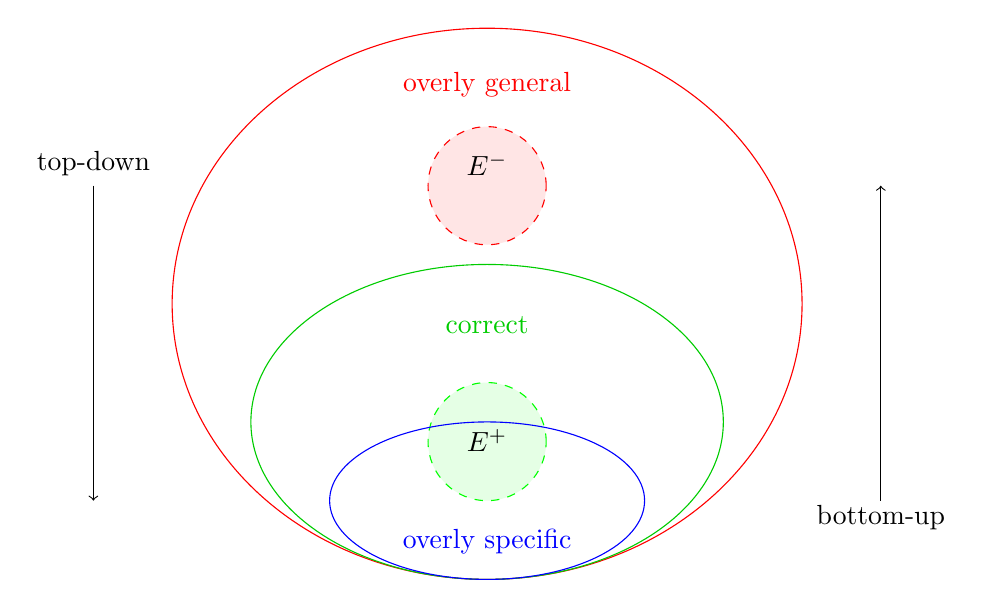
\begin{tikzpicture}
\draw[color=green, style=dashed, fill=green!10] (7, 1.75) circle (0.75);
\draw[color=red, style=dashed, fill=red!10] (7, 5) circle (0.75);
\draw[color=red] (7,3.5) ellipse (4 and 3.5);
\draw[color=green!80!black] (7,2) ellipse (3 and 2);
\draw[color=blue] (7,1) ellipse (2 and 1);
\fill (7,1.5) node[above] {$E^+$};
\fill (7,5) node[above] {$E^-$};
\fill[color=red] (7,6) node[above] {overly general};
\fill[color=green!80!black] (7,3) node[above] {correct};
\fill[color=blue] (7,0.2) node[above] {overly specific};
\draw [->] (12,1) -- (12,5);
\draw [->] (2,5) -- (2,1);
\fill (2,5) node[above] {top-down};
\fill (12,0.5) node[above] {bottom-up};
\end{tikzpicture}
\end{center}

\paragraph{Progol}
Progol searches top-down for hypotheses that subsume some bottom clause.\cite{nienhuys1997foundations}.
\paragraph{Aleph\cite{aleph2007}}
Although Aleph being based on Progol, it searches a hypothesis bottom-up. It first selects an example to be generalized, finds a bottom clause that entails it, then it generalizes the bottom clause further until a correct hypothesis is found.
\paragraph{Toplog\cite{muggleton2008toplog}}
Corapi\cite{corapi2011nonmonotonic} surveys that Toplog derives all the hypotheses $H_e$ that are generalizations of some positive example $e \in E^+$ constructing a set $H_c=\{h_e:e \in E^+\}$.
Afterwards a subset $H \in H_c$ maximizing a score function is chosen. Strictly in this sense Toplog does not perform a search. The first step of generalization is analogous to a bottom-up search. Based on the score function the second step of selection may eliminate overly general hypotheses and is therefore analogous to a top-down search. We conclude that Toplog uses a mixed hypothesis search strategy.
\paragraph{Xhail\cite{ray2003hybrid}}
Xhail (based on Hail) constructs a kernel set from the background knowledge $B$ and an example $e$ which is subsequently generalized until a correct hypothesis is found. Therefore Xhail searches a hypothesis $H$ bottom-up.

\paragraph{Imparo}
Imparo is based on the induction on failure (IoF) framework:
\begin{quote}\cite{kimber2012learning}
The procedure[IoF] interleaves top-down subsumption-based search with bottom-up generalisation of the ground connected theory T .
\end{quote}
Therefore Imparo uses a mixed strategy to search for a hypothesis.
\paragraph{Tal}
We conclude that Tal searches a hypothesis top-down from the quote bellow:
\begin{quote}\cite{corapi2010inductive}
Tal explores candidate solutions in a top-down manner,
backtracking whenever the current solution leads to failure in the abductive derivation.
\end{quote}

\section{Robustness}
We classify ILP systems based on whether they check for the consistency of the input theories and whether they always terminated.

\begin{center}
\captionof{table}{Classification by robustness} \label{tab:title} 
\begin{tabular}{| l | l | l | l | l | l | l |}
    \hline
    ILP system & Progol & Aleph & Toplog & Xhail & Imparo & Tal \\ \hline
    Consistency check & yes & no & no & yes & no & no \\
	& \ref{progol_consistency_check}
	& \ref{aleph_consistency_assumption}
	& \ref{toplog_consistency_assumption}
	 & \ref{xhail_implicit_consistency_check}
	 & \ref{imparo_consistency_assumption}
	 & \ref{tal_consistency_assumption} \\ \hline
    Always terminated & yes & yes & yes & yes & no & no \\ 
	&  & & & & \ref{imparo_clausal_examples} & \ref{tal_loop_on_learning_regular_languages} \\ \hline
\end{tabular}
\end{center} 

The property ``Always terminated'' evaluates whether an ILP system terminated on all the experiments in the appendix. However, it may be possible for a system that withstood our experiments that one could find an input on which a system would not terminate. Therefore this test is only indicative.